%% ------------------------------------------------------------------------- %%
\chapter{Introdução}

\noindent É comum em vários órgãos públicos a existência de diversos problemas de infraestrutura que ficam muito tempo sem solução devido a burocracia existente na abertura e encaminhamento de uma solicitação de reparo ou substituição de patrimônio.
Um motivo para os atrasos é o fato de que as informações sobre os setores responsáveis por determinadas atividades de uma organização, geralmente, não estão disponíveis de forma clara ao público, o que gera, em alguns casos, reclamações a órgãos ou departamentos cuja solicitação não é de sua competência.

A utilização de sistemas de \textit{internet} e aplicativos móveis podem amenizar a ocorrência de erros na comunicação entre reclamante e setor responsável pela manutenção do serviço, onde sua utilização em conjunto com uma central de atendimento, proporciona um canal direto de comunicação entre solicitante e a administração do serviço que fará o encaminhamento da solicitação para o órgão ou departamento responsável pelo atendimento. 

O motivo da crescente demanda referente a criação de aplicativos móveis no Brasil deve-se ao fato do povo brasileiro estar cada vez mais conectado à \textit{internet} através de aparelhos celulares. Segundo pesquisa feita em 2015 pela \gls{fgveasp} \cite{pesquisa-fgv}, a quantidade de \textit{smartphones} acaba de ultrapassar o número total de computadores em uso no país totalizando 154 milhões de aparelhos contra 152 milhões de computadores, que representam no total cerca de 306 milhões de dispositivos conectáveis a \textit{internet}.

O uso da tecnologia tem proporcionado melhoras na comunicação e produtividade no dia a dia das pessoas, o que fez com que criasse uma alta dependência da disponibilidade dos serviços de \gls{ti} pelos usuários fazendo com que as empresas buscassem novas maneiras de como manterem seus serviços disponíveis de forma a satisfazer as necessidades de seus clientes \cite{introductoryoverviewofitil}. Para que ocorra uma gerência eficaz em relação a disponibilidade dos serviços de \acrshort{ti}, foram criadas diversas ferramentas que têm como propósito fornecer um conjunto de recomendações para a governança e gerenciamento de serviços, dentre elas, o \gls{cobit}\footnote{COBIT: \textit{Control Objectives for Information and related Technology} \cite{bernard2012cobit}.}, \gls{cmmi}\footnote{CMMI: \textit{Capability Maturity Model Integration} \cite{Chrissis:2003:CGP:773274}}, a norma \gls{iso} 9001:2000\footnote{ISO 9001:2000: Norma internacional para gestão de serviços de \acrshort{ti}\cite{servicestrategy}.} e a biblioteca \gls{itil}, que é utilizada como base para construção deste trabalho \cite{abreu2012implantando, servicestrategy}.

%% ------------------------------------------------------------------------- %%
\section{Descrição do Problema}

\noindent O Campus Universitário de Palmas da \gls{uft} tem a sua infraestrutura organizada em blocos, estes são divididos em salas de aula, salas de professores, laboratórios, estações experimentais e ambientes administrativos \cite{infra-uft}. A Figura \ref{fig-campus-palmas} apresenta o mapa do Campus de Palmas da \acrshort{uft}.

\begin{figure}[!h]
  \centering
  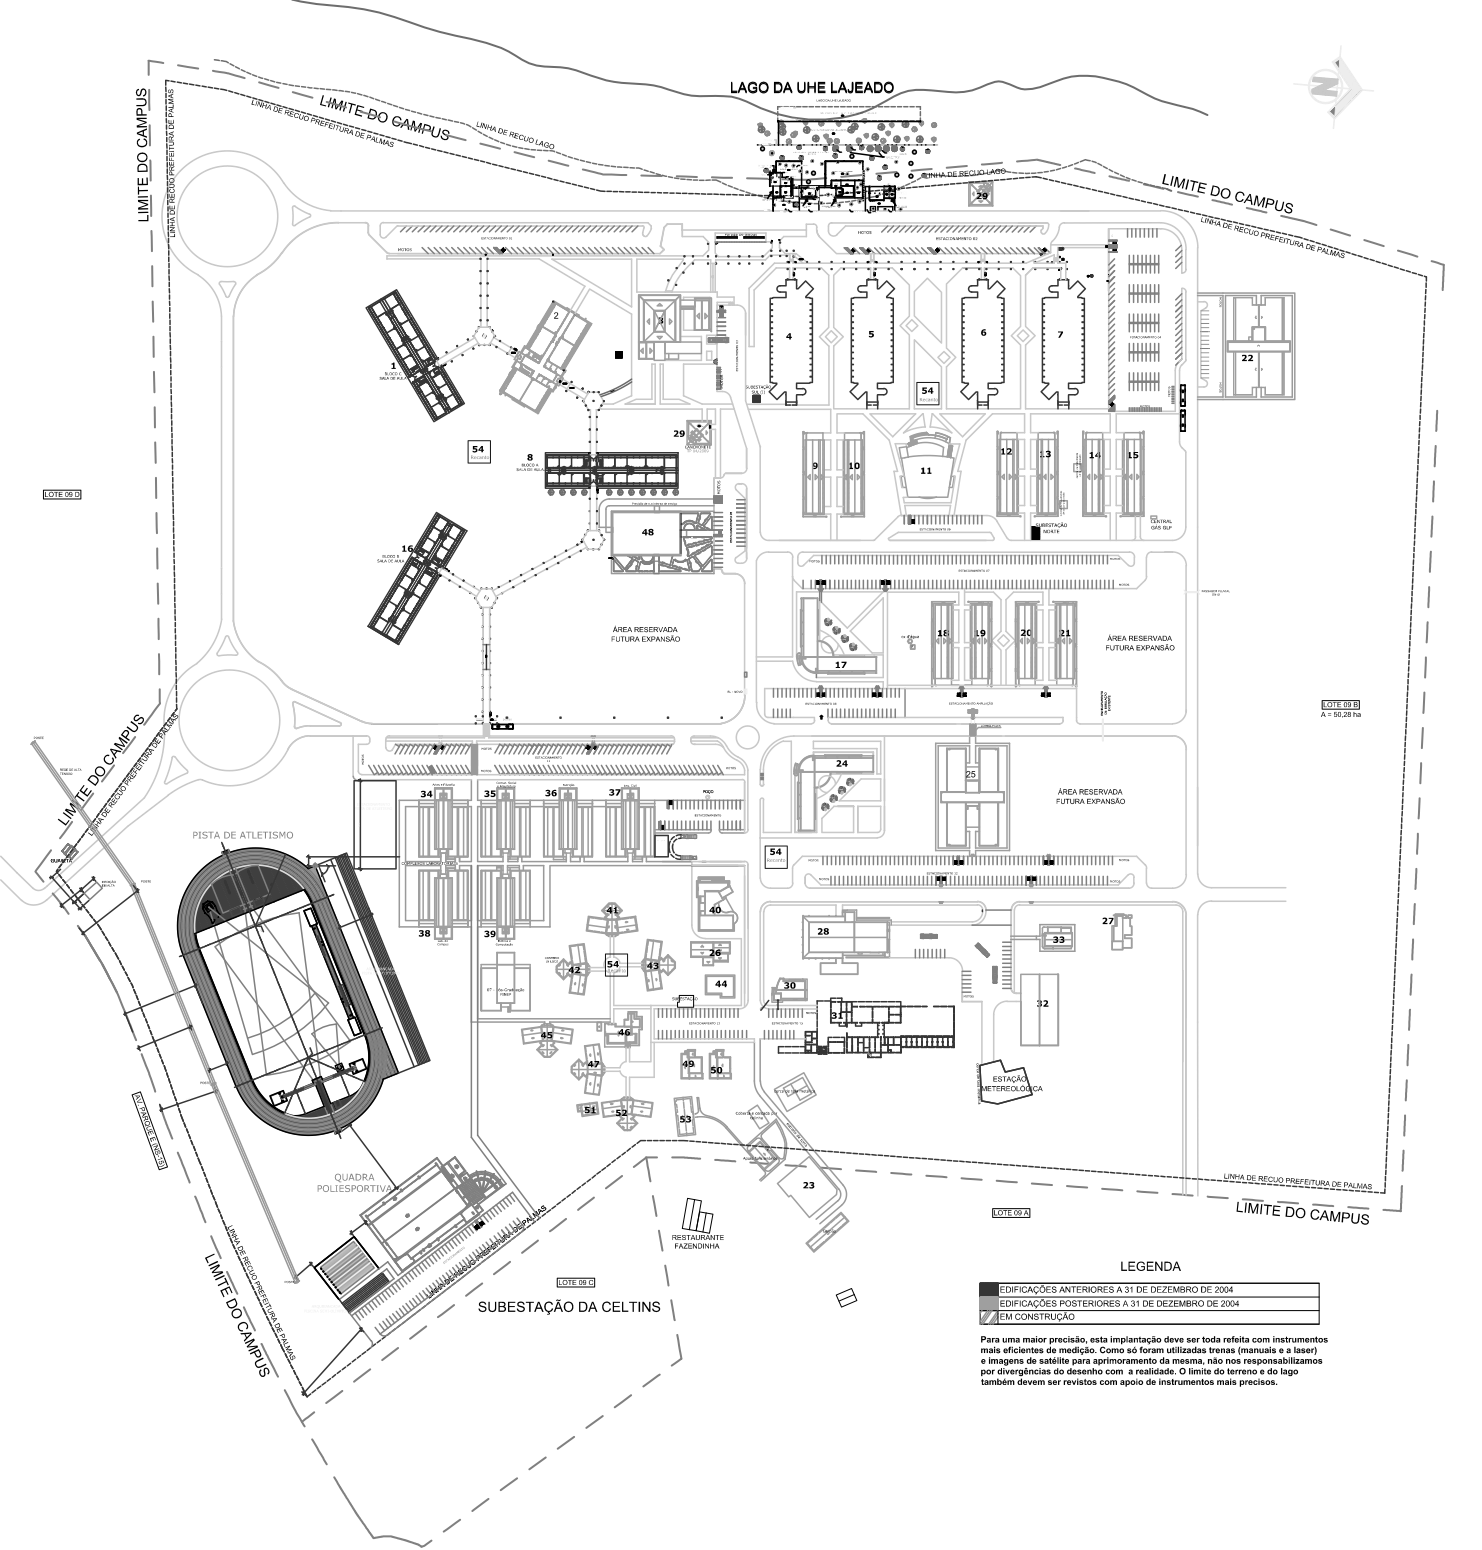
\includegraphics[width=.75\textwidth]{figuras/mapa.png} 
  \caption{Campus Universitário de Palmas da \acrshort{uft}.}
  \label{fig-campus-palmas} 
\end{figure}

A comunidade acadêmica da \acrshort{uft} é composta por três principais classes atuantes, sendo elas corpo docente, discente e técnico administrativo. Segundo pesquisa feita com o setor de \gls{rh} e a Secretaria Acadêmica do Campus Universitário de Palmas, é constatado em números a quantidade de alunos, professores e técnicos, sendo respectivamente 8118 alunos, 445 professores e 185 técnicos administrativos de acordo com o Anexo I e Anexo II. Conforme dados fornecidos pela Prefeitura Universitária, atualmente a infraestrutura do Campus de Palmas da \acrshort{uft} é formada por 53 blocos.

Diariamente diversos recursos da universidade são utilizados pelo corpo docente, discente e administrativo do campus com o objetivo de propiciar a manutenção e o funcionamento adequado das atividades realizadas na universidade. Mas, com o decorrer do tempo, algumas adversidades podem surgir com sua infraestrutura, sendo recorrente o surgimento de problemas como o mau funcionamento de aparelhos de ar condicionado, infiltração nas salas de aula em época de chuva, problemas com a iluminação entre blocos e o não funcionamento adequado dos sanitários e bebedouros.

A deterioração dos pertences da universidade prejudica o andamento das atividades realizadas no campus universitário, sendo que normalmente a formalização de pedidos de reparo são feitos via telefone ou pelo envio de \textit{e-mail} e memorandos, o que dificulta e burocratiza o processo de abertura de chamados pela comunidade acadêmica.

Atualmente, diversos sistemas propõem uma solução para solicitação de reparos, como o Alô Pequi \cite{alo_pequi} usado pela prefeitura da cidade de Palmas no estado do Tocantins e o Colab \cite{colab} que é utilizado por várias prefeituras no Brasil. A \acrshort{uft} dispõe, atualmente, de  um sistema \textit{web} para o gerenciamento de ordens de serviço chamado \gls{mandi} (Monitoramento e Análise de Incidentes) em sua \textit{intranet}, cujo o funcionamento consiste na criação e listagem de solicitação de reparo, entretanto, a abertura e encaminhamento são feitos apenas pelos funcionários da universidade.

A Figura \ref{fig-mandi-uft} mostra a tela inicial do sistema  \acrshort{mandi}. Uma característica negativa notada no sistema é o fato de sua utilização estar restrita à sua interface \textit{web}, além de não haver uma adaptação para resolução de tela de dispositivos móveis, o que dificulta a sua utilização por aparelhos como \textit{smartphones} e \textit{tablets}. Outro ponto negativo do sistema é o fato do seu acesso estar restrito apenas aos funcionários com suas devidas permissão, o que impossibilita a abertura de chamados por parte dos alunos e professores. O atual sistema não provê uma ferramenta para geração de relatórios o que dificulta o processo de análise e auditoria sobre as ocorrências e encaminhamentos realizado pelos atendentes do sistema, tornando assim uma menor transparência das políticas adotadas para o atendimento das solicitações com relação a comunidade acadêmica.

\begin{figure}[!h]
  \centering
  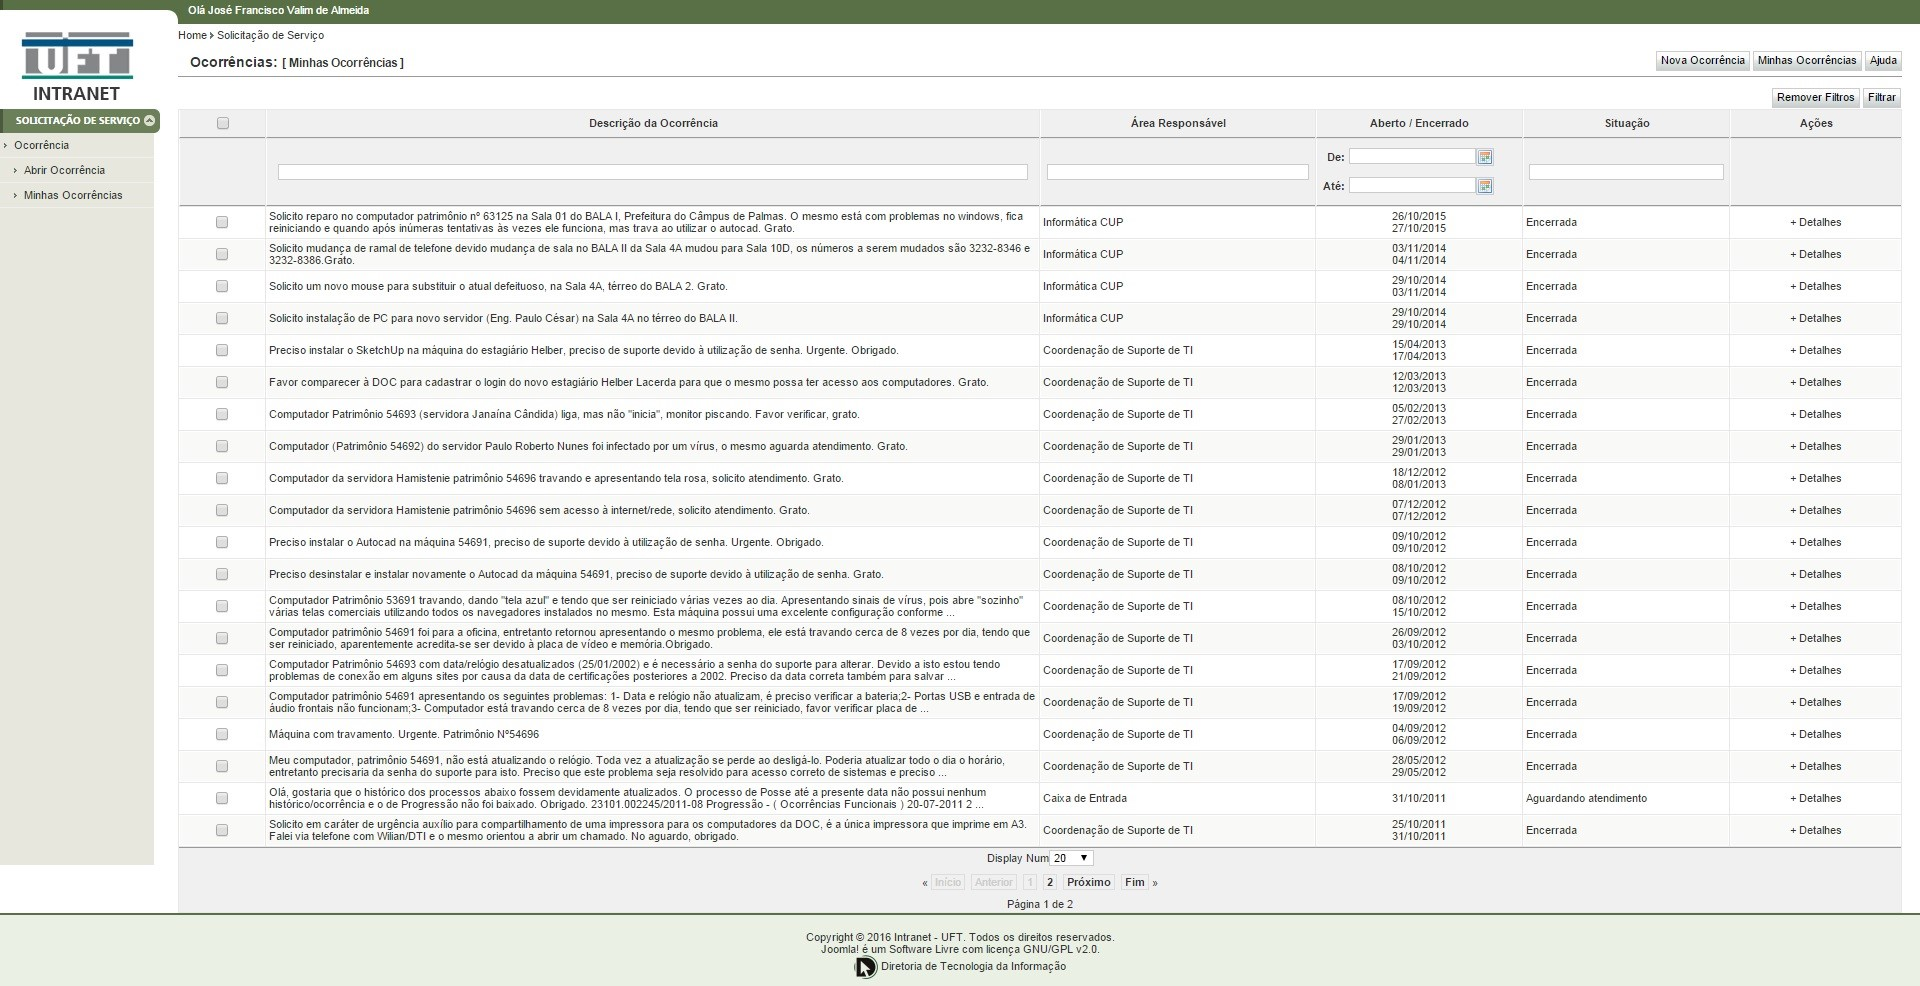
\includegraphics[width=1\textwidth]{figuras/tela-inicial-mandi.jpg}
  \caption{Tela inicial sistema \acrshort{mandi} (Adaptada de \cite{intranet_uft}).}
  \label{fig-mandi-uft} 
\end{figure}

O sistema apresenta um grave problema relacionado com a precisão dos dados referentes ao local de abertura do chamado e as informações pessoais do solicitante, erro que é cometido, pois, o programa possibilita a abertura de chamados sem que haja uma correta especificação dos dados do local do problema e das informações pessoais do solicitante. 
Existem alguns pontos com relação a falha de análise dos requisitos do sistema, um deles é o fato que a vinculação da responsabilidade da abertura do chamado fica apenas sobre a responsabilidade do atendente e não havendo a possibilidade de vinculação ao departamento responsável pelo encaminhamento da solicitação. Outra falha está na falta da possibilidade de encaminhamento por \textit{e-mail} das solicitações de ordem de serviços para os setores/empresas responsáveis através do sistema, o que torna um trabalho manual o envio dos encaminhamentos das ordem de serviços dificultando assim o andamento da solução do problema.

%% ------------------------------------------------------------------------- %%
\section{Justificativa}

\noindent Ao observar as possibilidades que a \textit{internet} oferece, tais como os recursos para comunicação através de dispositivos móveis \cite{pesquisa-fgv}, verificou-se o grande potencial que o uso de aplicativos (embarcados em \textit{smartphones} e \textit{tablets}) tem em proporcionar uma troca rápida e eficaz de informações entre pessoas.
Diante da necessidade de criar um sistema de gerenciamento de manutenção de serviços no Campus Universitário de Palmas da \acrshort{uft}, constatou-se a oportunidade de implantação de uma aplicação móvel para abertura e acompanhamento de chamados intitulada ``\acrshort{uft} Serviços''. O \textit{software} consiste em um aplicativo para solicitação de ordem de serviço e uma interface \textit{web} para gerenciamento dos atendimentos requisitados através do aplicativo móvel.

Para implantação do sistema ``\acrshort{uft} Serviços'' são utilizadas as especificações do \gls{itil} v3 como modelo de implantação de serviços, em razão dos benefícios que a especificação proporciona através de sua coletânea de informações contendo recomendações para o gerenciamento de serviços de \acrshort{ti} \cite{introductoryoverviewofitil}.

Uma das motivações para a escolha do \gls{itil} como modelo de gerenciamento de serviços de \acrshort{ti} é a sua ampla utilização por diversos setores e empresas ao redor do mundo, dentre as mais famosas \cite{arraj2010itil}:

\begin{itemize}
    \item Grandes empresas da área de tecnologia como Microsoft, \gls{hp}, Fujitsu e \gls{ibm};
    \item Empresas varejistas como a Target, Walmart e Staples;
    \item Organizações de serviços financeiros como o Citi, \textit{Bank of America} e o \textit{Barclay's Bank};
    \item Empresas de entretenimento como a Disney e Sony;
    \item Fabricantes como a Boeing, Toyota e Bomdardier; e
    \item Empresas da área de ciência da vida, como a Eli Lilly, Pfizer e Takeda Phamaceuticals.
\end{itemize}

Nesse contexto, a aplicação ``\acrshort{uft} Serviços'' visa sobretudo tornar mais fácil a comunicação entre a comunidade acadêmica e a administração do campus com relação aos eventuais problemas de infraestrutura presentes no campus universitário, agilizando os processos de abertura de chamados e diminuindo assim o tempo necessário para que setores responsáveis sejam notificados sobre as solicitações.

\section*{Uso de Aplicativos Móveis}

\noindent A utilização de soluções de aplicações móveis está cada vez mais presente no cotidiano das pessoas e sua ampla utilização deve-se as vantagens significativas que a utilização de aplicativos para \textit{smartphones} fornece aos seus usuários, dentre elas destaca-se a portabilidade, reconhecimento de local e acessibilidade de acesso a informação \cite{nayebi2012state}.

O mercado de \textit{smartphones} encontra-se focado em três principais plataformas de desenvolvimento:  \textit{Android}, \gls{ios} e Windows Phone. A plataforma \textit{Android} domina o mercado mundial de dispositivos móveis, segundo dados da \gls{idc}, em agosto de 2015 a plataforma representa 82\% do \textit{market share} dos \textit{smartphones} no mundo, seguido pelo sistema operacional \acrshort{ios} que tem aproximadamente 13.9\% \cite{pesquisa-idc}.

Atualmente, diversos modelos de desenvolvimento para dispositivos móveis são utilizados, sendo eles o modelo nativo, híbrido e \textit{web} \cite{charland2011mobile}. O modelo nativo é o mais conhecido dentre os demais, sua principal vantagem está no fato dos aplicativos utilizam todos os recursos fornecidos pelo \textit{hardware} do aparelho além de oferecer boa performance. A desvantagem de sua utilização fica por conta da curva de aprendizado e o custo de manutenção do sistema, pois para cada sistema operacional é utilizado linguagens e \textit{frameworks} específicos o que impossibilita uma convergência do uso do mesmo código para mais de uma plataforma \cite{charland2011mobile}.

Já o modelo \textit{web} é uma proposta que utiliza como meio de desenvolvimento ferramentas já conhecidas do desenvolvimento de sistema para \textit{internet} como \gls{html}, Java Script e \gls{css}, sua principal vantagem tem como motivo que diversos \textit{frameworks} disponíveis no mercado permitem a convergência do mesmo aplicativos para diferentes plataformas. A principal desvantagem do uso desse modelo fica por conta da limitação de acesso ao \textit{hardware} e baixa performance que o tipo de desenvolvimento proporciona \cite{charland2011mobile}.

Mais recentemente surgiu em resposta a necessidade de convergência de plataformas de um mesmo aplicativo o modelo híbrido, sua principal característica fica pelo fato de proporcionar boa performance utilizando uma mesma linguagem de programação e \textit{framework} para geração de código nativo para diversas plataformas móveis \cite{charland2011mobile}.

%% ------------------------------------------------------------------------- %%

\section{Objetivos}

\noindent Para um melhor entendimento dos objetivos alcançados neste trabalho, os objetivos foram
divididos em objetivos gerais e objetivos específicos, mostrados a seguir.

%% ------------------------------------------------------------------------- %%
\subsection{Objetivo Geral}

\noindent O objetivo principal deste trabalho consiste no desenvolvimento e implantação de um sistema para manutenção de serviços intitulado ``\acrshort{uft} Serviços'', utilizando as diretrizes do \gls{itil} v3 para o gerenciamento dos processos de \acrshort{ti}. 

O principal propósito do desenvolvimento deste sistema está em atender as necessidades do Campus Universitário de Palmas da \acrshort{uft} quanto a introdução de um sistema para abertura e gerenciamento de chamados que seja de alcance amplo por toda a comunidade acadêmica (docente, discente e técnico administrativo). 

Procura-se através da utilização do \acrshort{itil} e de boas práticas de desenvolvimento de \textit{software} garantir, a disponibilidade, segurança e a continuidade dos serviços oferecidos pelo sistema através da possibilidade da inclusão de novos requisitos que sejam necessários para que ocorra a manutenção dos serviços oferecidos pelo sistema de maneira eficiente.

%% ------------------------------------------------------------------------- %%  
\subsection{Objetivos Específicos}

\begin{enumerate}
    \item Desenvolver aplicação móvel para a plataforma \textit{Android} a fim de ampliar o alcance de sua utilização;
    \item Implantar uma aplicação \textit{web} em forma de \textit{dashboard} para acompanhamento, atendimento e geração de relatórios analíticos sobre os problemas catalogados no sistema;
    \item Executar testes de segurança, desempenho e lançamento de beta testes para implantação do ``\acrshort{uft} Serviços'';
    \item Garantir que o sistema comporte um número mínimo de conexões simultâneas que atenda o uso do sistema pela comunidade acadêmica do Campus de Palmas;
    \item Utilizar técnicas de teste de usabilidade de \textit{software} a fim mensurar a experiência do usuário com o sistema;
    \item Assegurar que o sistema seja tolerante a falhas, ofertando aos usuários a possibilidade de reportar erros;
    \item Utilizar as recomendações da etapa de Estratégia de Serviços do \gls{itil} afim de alinhar os serviços oferecidos pelo sistema com os objetivos da instituição;
    \item Projetar novas funcionalidades do sistema utilizando a etapa de Desenho de Serviços do \gls{itil};
    \item Utilizar as recomendações da etapa de Transição de Serviço a fim de garantir a introdução de novos recursos no sistema;
    \item Utilizar a metodologia de desenvolvimento ágil \textit{Scrum} como ferramenta de auxílio para o alcance dos requisitos do sistema; e
    \item Construir uma base sólida do sistema para que a atual equipe de desenvolvimento do campus dê continuidade ao serviço.
\end{enumerate}

%% ------------------------------------------------------------------------- %%
\section{Estrutura do Trabalho}

\noindent O \textbf{capítulo 2} apresenta a fundamentação teórica, na qual serão mostrados os conceitos utilizados para o desenvolvimento e implantação do sistema. Em seguida, no \textbf{capítulo 3}, é apresentado os Trabalhos Relacionados com enfoque em casos de sucesso da implantação do \gls{itil} na literatura além de mostrar sistemas de gerenciamento de manutenção de serviços já em produção, apresentando suas funcionalidades e fragilidades.  No \textbf{capítulo 4} é apresentado o capítulo de Metodologia, nele é apresentado informações sobre os métodos aplicados para a construção desta monografia. Em sequência no \textbf{capítulo 5} é apresentado os resultados obtidos pela implantação do sistema ``\acrshort{uft} Serviços''.
Por fim, no \textbf{capítulo 6} é apresentado o capítulo de Conclusão e Trabalhos Futuros onde são apresentados as conclusões obtidas pela finalização deste trabalho, bem como a apresentação de sugestões para trabalhos futuros e os resultados adicionais obtidos.